\documentclass[twoside]{book}

% Packages required by doxygen
\usepackage{fixltx2e}
\usepackage{calc}
\usepackage{doxygen}
\usepackage[export]{adjustbox} % also loads graphicx
\usepackage{graphicx}
\usepackage[utf8]{inputenc}
\usepackage{makeidx}
\usepackage{multicol}
\usepackage{multirow}
\PassOptionsToPackage{warn}{textcomp}
\usepackage{textcomp}
\usepackage[nointegrals]{wasysym}
\usepackage[table]{xcolor}

% Font selection
\usepackage[T1]{fontenc}
\usepackage[scaled=.90]{helvet}
\usepackage{courier}
\usepackage{amssymb}
\usepackage{sectsty}
\renewcommand{\familydefault}{\sfdefault}
\allsectionsfont{%
  \fontseries{bc}\selectfont%
  \color{darkgray}%
}
\renewcommand{\DoxyLabelFont}{%
  \fontseries{bc}\selectfont%
  \color{darkgray}%
}
\newcommand{\+}{\discretionary{\mbox{\scriptsize$\hookleftarrow$}}{}{}}

% Page & text layout
\usepackage{geometry}
\geometry{%
  a4paper,%
  top=2.5cm,%
  bottom=2.5cm,%
  left=2.5cm,%
  right=2.5cm%
}
\tolerance=750
\hfuzz=15pt
\hbadness=750
\setlength{\emergencystretch}{15pt}
\setlength{\parindent}{0cm}
\setlength{\parskip}{3ex plus 2ex minus 2ex}
\makeatletter
\renewcommand{\paragraph}{%
  \@startsection{paragraph}{4}{0ex}{-1.0ex}{1.0ex}{%
    \normalfont\normalsize\bfseries\SS@parafont%
  }%
}
\renewcommand{\subparagraph}{%
  \@startsection{subparagraph}{5}{0ex}{-1.0ex}{1.0ex}{%
    \normalfont\normalsize\bfseries\SS@subparafont%
  }%
}
\makeatother

% Headers & footers
\usepackage{fancyhdr}
\pagestyle{fancyplain}
\fancyhead[LE]{\fancyplain{}{\bfseries\thepage}}
\fancyhead[CE]{\fancyplain{}{}}
\fancyhead[RE]{\fancyplain{}{\bfseries\leftmark}}
\fancyhead[LO]{\fancyplain{}{\bfseries\rightmark}}
\fancyhead[CO]{\fancyplain{}{}}
\fancyhead[RO]{\fancyplain{}{\bfseries\thepage}}
\fancyfoot[LE]{\fancyplain{}{}}
\fancyfoot[CE]{\fancyplain{}{}}
\fancyfoot[RE]{\fancyplain{}{\bfseries\scriptsize Generated by Doxygen }}
\fancyfoot[LO]{\fancyplain{}{\bfseries\scriptsize Generated by Doxygen }}
\fancyfoot[CO]{\fancyplain{}{}}
\fancyfoot[RO]{\fancyplain{}{}}
\renewcommand{\footrulewidth}{0.4pt}
\renewcommand{\chaptermark}[1]{%
  \markboth{#1}{}%
}
\renewcommand{\sectionmark}[1]{%
  \markright{\thesection\ #1}%
}

% Indices & bibliography
\usepackage{natbib}
\usepackage[titles]{tocloft}
\setcounter{tocdepth}{3}
\setcounter{secnumdepth}{5}
\makeindex

% Hyperlinks (required, but should be loaded last)
\usepackage{ifpdf}
\ifpdf
  \usepackage[pdftex,pagebackref=true]{hyperref}
\else
  \usepackage[ps2pdf,pagebackref=true]{hyperref}
\fi
\hypersetup{%
  colorlinks=true,%
  linkcolor=blue,%
  citecolor=blue,%
  unicode%
}

% Custom commands
\newcommand{\clearemptydoublepage}{%
  \newpage{\pagestyle{empty}\cleardoublepage}%
}

\usepackage{caption}
\captionsetup{labelsep=space,justification=centering,font={bf},singlelinecheck=off,skip=4pt,position=top}

%===== C O N T E N T S =====

\begin{document}

% Titlepage & ToC
\hypersetup{pageanchor=false,
             bookmarksnumbered=true,
             pdfencoding=unicode
            }
\pagenumbering{alph}
\begin{titlepage}
\vspace*{7cm}
\begin{center}%
{\Large Projet R\&D }\\
\vspace*{1cm}
{\large Generated by Doxygen 1.8.14}\\
\end{center}
\end{titlepage}
\clearemptydoublepage
\pagenumbering{roman}
\tableofcontents
\clearemptydoublepage
\pagenumbering{arabic}
\hypersetup{pageanchor=true}

%--- Begin generated contents ---
\chapter{Hierarchical Index}
\section{Class Hierarchy}
This inheritance list is sorted roughly, but not completely, alphabetically\+:\begin{DoxyCompactList}
\item \contentsline{section}{Algorithm\+Controller.\+Algorithm\+Controller}{\pageref{class_algorithm_controller_1_1_algorithm_controller}}{}
\item \contentsline{section}{Ant\+Model.\+Ant\+Model}{\pageref{class_ant_model_1_1_ant_model}}{}
\item \contentsline{section}{Building\+Model.\+Building\+Model}{\pageref{class_building_model_1_1_building_model}}{}
\item \contentsline{section}{Care\+Model.\+Care\+Model}{\pageref{class_care_model_1_1_care_model}}{}
\item \contentsline{section}{File\+Controller.\+File\+Controller}{\pageref{class_file_controller_1_1_file_controller}}{}
\item \contentsline{section}{Instance\+Controller.\+Instance\+Controller}{\pageref{class_instance_controller_1_1_instance_controller}}{}
\item \contentsline{section}{Instance\+Model.\+Instance\+Model}{\pageref{class_instance_model_1_1_instance_model}}{}
\item \contentsline{section}{Pheromone\+Model.\+Pheromone\+Model}{\pageref{class_pheromone_model_1_1_pheromone_model}}{}
\item \contentsline{section}{Probability\+Controller.\+Probability\+Controller}{\pageref{class_probability_controller_1_1_probability_controller}}{}
\item \contentsline{section}{Solution\+Model.\+Solution\+Model}{\pageref{class_solution_model_1_1_solution_model}}{}
\item Test\+Case\begin{DoxyCompactList}
\item \contentsline{section}{Test\+Algorithm\+Controller.\+Test\+Algorithm\+Controller}{\pageref{class_test_algorithm_controller_1_1_test_algorithm_controller}}{}
\item \contentsline{section}{Test\+File\+Controller.\+Test\+File\+Controller}{\pageref{class_test_file_controller_1_1_test_file_controller}}{}
\item \contentsline{section}{Test\+Instance\+Controller.\+Test\+Instance\+Controller}{\pageref{class_test_instance_controller_1_1_test_instance_controller}}{}
\item \contentsline{section}{Test\+Probability\+Controller.\+calculate\+Probability}{\pageref{class_test_probability_controller_1_1calculate_probability}}{}
\end{DoxyCompactList}
\item \contentsline{section}{Test\+Parameters.\+Test\+Parameters}{\pageref{class_test_parameters_1_1_test_parameters}}{}
\item \contentsline{section}{Test\+Solution.\+Test\+Solution}{\pageref{class_test_solution_1_1_test_solution}}{}
\item Pheromone\+Model\begin{DoxyCompactList}
\item \contentsline{section}{Pheromone\+Edge.\+Pheromone\+Edge}{\pageref{class_pheromone_edge_1_1_pheromone_edge}}{}
\item \contentsline{section}{Pheromone\+Node.\+Pheromone\+Node}{\pageref{class_pheromone_node_1_1_pheromone_node}}{}
\end{DoxyCompactList}
\end{DoxyCompactList}

\chapter{Class Index}
\section{Class List}
Here are the classes, structs, unions and interfaces with brief descriptions\+:\begin{DoxyCompactList}
\item\contentsline{section}{\mbox{\hyperlink{class_algorithm_controller_1_1_algorithm_controller}{Algorithm\+Controller.\+Algorithm\+Controller}} }{\pageref{class_algorithm_controller_1_1_algorithm_controller}}{}
\item\contentsline{section}{\mbox{\hyperlink{class_ant_model_1_1_ant_model}{Ant\+Model.\+Ant\+Model}} }{\pageref{class_ant_model_1_1_ant_model}}{}
\item\contentsline{section}{\mbox{\hyperlink{class_building_model_1_1_building_model}{Building\+Model.\+Building\+Model}} }{\pageref{class_building_model_1_1_building_model}}{}
\item\contentsline{section}{\mbox{\hyperlink{class_test_probability_controller_1_1calculate_probability}{Test\+Probability\+Controller.\+calculate\+Probability}} }{\pageref{class_test_probability_controller_1_1calculate_probability}}{}
\item\contentsline{section}{\mbox{\hyperlink{class_care_model_1_1_care_model}{Care\+Model.\+Care\+Model}} }{\pageref{class_care_model_1_1_care_model}}{}
\item\contentsline{section}{\mbox{\hyperlink{class_file_controller_1_1_file_controller}{File\+Controller.\+File\+Controller}} }{\pageref{class_file_controller_1_1_file_controller}}{}
\item\contentsline{section}{\mbox{\hyperlink{class_instance_controller_1_1_instance_controller}{Instance\+Controller.\+Instance\+Controller}} }{\pageref{class_instance_controller_1_1_instance_controller}}{}
\item\contentsline{section}{\mbox{\hyperlink{class_instance_model_1_1_instance_model}{Instance\+Model.\+Instance\+Model}} }{\pageref{class_instance_model_1_1_instance_model}}{}
\item\contentsline{section}{\mbox{\hyperlink{class_pheromone_edge_1_1_pheromone_edge}{Pheromone\+Edge.\+Pheromone\+Edge}} }{\pageref{class_pheromone_edge_1_1_pheromone_edge}}{}
\item\contentsline{section}{\mbox{\hyperlink{class_pheromone_model_1_1_pheromone_model}{Pheromone\+Model.\+Pheromone\+Model}} }{\pageref{class_pheromone_model_1_1_pheromone_model}}{}
\item\contentsline{section}{\mbox{\hyperlink{class_pheromone_node_1_1_pheromone_node}{Pheromone\+Node.\+Pheromone\+Node}} }{\pageref{class_pheromone_node_1_1_pheromone_node}}{}
\item\contentsline{section}{\mbox{\hyperlink{class_probability_controller_1_1_probability_controller}{Probability\+Controller.\+Probability\+Controller}} }{\pageref{class_probability_controller_1_1_probability_controller}}{}
\item\contentsline{section}{\mbox{\hyperlink{class_solution_model_1_1_solution_model}{Solution\+Model.\+Solution\+Model}} }{\pageref{class_solution_model_1_1_solution_model}}{}
\item\contentsline{section}{\mbox{\hyperlink{class_test_algorithm_controller_1_1_test_algorithm_controller}{Test\+Algorithm\+Controller.\+Test\+Algorithm\+Controller}} }{\pageref{class_test_algorithm_controller_1_1_test_algorithm_controller}}{}
\item\contentsline{section}{\mbox{\hyperlink{class_test_file_controller_1_1_test_file_controller}{Test\+File\+Controller.\+Test\+File\+Controller}} }{\pageref{class_test_file_controller_1_1_test_file_controller}}{}
\item\contentsline{section}{\mbox{\hyperlink{class_test_instance_controller_1_1_test_instance_controller}{Test\+Instance\+Controller.\+Test\+Instance\+Controller}} }{\pageref{class_test_instance_controller_1_1_test_instance_controller}}{}
\item\contentsline{section}{\mbox{\hyperlink{class_test_parameters_1_1_test_parameters}{Test\+Parameters.\+Test\+Parameters}} }{\pageref{class_test_parameters_1_1_test_parameters}}{}
\item\contentsline{section}{\mbox{\hyperlink{class_test_solution_1_1_test_solution}{Test\+Solution.\+Test\+Solution}} }{\pageref{class_test_solution_1_1_test_solution}}{}
\end{DoxyCompactList}

\chapter{Class Documentation}
\hypertarget{class_algorithm_controller_1_1_algorithm_controller}{}\section{Algorithm\+Controller.\+Algorithm\+Controller Class Reference}
\label{class_algorithm_controller_1_1_algorithm_controller}\index{Algorithm\+Controller.\+Algorithm\+Controller@{Algorithm\+Controller.\+Algorithm\+Controller}}
\subsection*{Public Member Functions}
\begin{DoxyCompactItemize}
\item 
def \mbox{\hyperlink{class_algorithm_controller_1_1_algorithm_controller_a2f8217779ecd4b8ffbcb6869a8abf5ef}{\+\_\+\+\_\+init\+\_\+\+\_\+}} (self, instance, care\+Effect\+Radius)
\item 
def \mbox{\hyperlink{class_algorithm_controller_1_1_algorithm_controller_a16c94d71907fe272accefc3b11d202ef}{run}} (self, iteration\+Times)
\item 
def \mbox{\hyperlink{class_algorithm_controller_1_1_algorithm_controller_aceaf2f248880e85bebd1d1c5a3ee50e2}{allocate\+Building}} (self, ant, copy\+Distance\+Sorted\+Building\+Index\+Matrix, solution\+For\+One\+Iteration\+List, quality\+Of\+Solution\+For\+One\+Iteration\+List)
\item 
def \mbox{\hyperlink{class_algorithm_controller_1_1_algorithm_controller_a3e4df24f596b73789fe10ef001dc4fd7}{choose\+Care}} (self, buidling\+To\+Allocate\+Index, building\+To\+Allocate\+List, care\+To\+Fill\+List, is\+Care\+Full\+List, solution)
\item 
def \mbox{\hyperlink{class_algorithm_controller_1_1_algorithm_controller_a6be8ad6c0ed5d3733cc3678f4e73a6f5}{sort\+Building\+Index\+For\+Each\+Care\+In\+Distance\+Matrix}} (self)
\item 
def \mbox{\hyperlink{class_algorithm_controller_1_1_algorithm_controller_a93353daa1fde6df34d6b22af6a773610}{merge\+\_\+sort}} (self, distance\+List, distance\+Index\+List)
\item 
def \mbox{\hyperlink{class_algorithm_controller_1_1_algorithm_controller_a93b60c2a1787e8d5c3f940ddd6d051e9}{objective\+FunctionF}} (self, solution)
\item 
def \mbox{\hyperlink{class_algorithm_controller_1_1_algorithm_controller_a96414bd12515fbd19bc103cbc0b9cdcb}{objective\+FunctionG}} (self, solution)
\item 
def \mbox{\hyperlink{class_algorithm_controller_1_1_algorithm_controller_abe539c495b1f651be7198f43c7640ce0}{objective\+FunctionH}} (self, solution)
\item 
def \mbox{\hyperlink{class_algorithm_controller_1_1_algorithm_controller_a6b570c9ebad1e6a937e74490fab6a8a9}{calculate\+Average\+Solution\+Quality\+For\+Each\+Iteration}} (self, quality\+Of\+Solution\+For\+One\+Iteration\+List)
\end{DoxyCompactItemize}
\subsection*{Public Attributes}
\begin{DoxyCompactItemize}
\item 
\mbox{\Hypertarget{class_algorithm_controller_1_1_algorithm_controller_ae5b0382b72120d0b7412baa3e59b2b82}\label{class_algorithm_controller_1_1_algorithm_controller_ae5b0382b72120d0b7412baa3e59b2b82}} 
{\bfseries instance}
\item 
\mbox{\Hypertarget{class_algorithm_controller_1_1_algorithm_controller_a562b9b093fd7ff0cfedb6b7a814e92f8}\label{class_algorithm_controller_1_1_algorithm_controller_a562b9b093fd7ff0cfedb6b7a814e92f8}} 
{\bfseries best\+Solution}
\item 
\mbox{\Hypertarget{class_algorithm_controller_1_1_algorithm_controller_a10c4b05a70d8fea5c86e4dd936f57914}\label{class_algorithm_controller_1_1_algorithm_controller_a10c4b05a70d8fea5c86e4dd936f57914}} 
{\bfseries care\+Effect\+Radius}
\end{DoxyCompactItemize}


\subsection{Detailed Description}
\begin{DoxyVerb}Description: cette classe est le controleur d'algorthime, qui réalise à chercher la meilleur solution d'affection
Attributs:
    instance: (l'objet de la classe InstanceModel) l'instance préparée par la classe InstanceControleur,
                y compris la liste de bâtiments,la liste de cares, la liste de phéromones sur les nœuds de bâtiment,
                la matrice de phéromones sur les arcs entre le bâtiment et le care,la liste de fourmis
    bestSolution: (l'objet de la classe SolutionModel) la meilleure solution trouvé finalement
    careEffectRadius: (int) le rayon d'attraction initial de circle dont le centre est chaque care
\end{DoxyVerb}
 

\subsection{Constructor \& Destructor Documentation}
\mbox{\Hypertarget{class_algorithm_controller_1_1_algorithm_controller_a2f8217779ecd4b8ffbcb6869a8abf5ef}\label{class_algorithm_controller_1_1_algorithm_controller_a2f8217779ecd4b8ffbcb6869a8abf5ef}} 
\index{Algorithm\+Controller\+::\+Algorithm\+Controller@{Algorithm\+Controller\+::\+Algorithm\+Controller}!\+\_\+\+\_\+init\+\_\+\+\_\+@{\+\_\+\+\_\+init\+\_\+\+\_\+}}
\index{\+\_\+\+\_\+init\+\_\+\+\_\+@{\+\_\+\+\_\+init\+\_\+\+\_\+}!Algorithm\+Controller\+::\+Algorithm\+Controller@{Algorithm\+Controller\+::\+Algorithm\+Controller}}
\subsubsection{\texorpdfstring{\+\_\+\+\_\+init\+\_\+\+\_\+()}{\_\_init\_\_()}}
{\footnotesize\ttfamily def Algorithm\+Controller.\+Algorithm\+Controller.\+\_\+\+\_\+init\+\_\+\+\_\+ (\begin{DoxyParamCaption}\item[{}]{self,  }\item[{}]{instance,  }\item[{}]{care\+Effect\+Radius }\end{DoxyParamCaption})}

\begin{DoxyVerb}Description: cette méthode est le constructeur de la classe AlgorithmeControlleur
:param instance: (l'objet de la classe InstanceModel) l'instance de programme,
            qui est préparée par la classe InstanceControleur
:param careEffectRadius: (int) le rayon d'attraction initial de chaque care, qui est définit par l'utilisateur
                    dans le script main.py
\end{DoxyVerb}
 

\subsection{Member Function Documentation}
\mbox{\Hypertarget{class_algorithm_controller_1_1_algorithm_controller_aceaf2f248880e85bebd1d1c5a3ee50e2}\label{class_algorithm_controller_1_1_algorithm_controller_aceaf2f248880e85bebd1d1c5a3ee50e2}} 
\index{Algorithm\+Controller\+::\+Algorithm\+Controller@{Algorithm\+Controller\+::\+Algorithm\+Controller}!allocate\+Building@{allocate\+Building}}
\index{allocate\+Building@{allocate\+Building}!Algorithm\+Controller\+::\+Algorithm\+Controller@{Algorithm\+Controller\+::\+Algorithm\+Controller}}
\subsubsection{\texorpdfstring{allocate\+Building()}{allocateBuilding()}}
{\footnotesize\ttfamily def Algorithm\+Controller.\+Algorithm\+Controller.\+allocate\+Building (\begin{DoxyParamCaption}\item[{}]{self,  }\item[{}]{ant,  }\item[{}]{copy\+Distance\+Sorted\+Building\+Index\+Matrix,  }\item[{}]{solution\+For\+One\+Iteration\+List,  }\item[{}]{quality\+Of\+Solution\+For\+One\+Iteration\+List }\end{DoxyParamCaption})}

\begin{DoxyVerb}Description: cette méthode est pour sélectionner les bâtiments à affecter
:param ant: (l'objet de la classe AntModel) un fourmi qui va chercher sa solution
:param copyDistanceSortedBuildingIndexMatrix: (int[][]) la matrice copièe d'indices de bâtiment référée la matrice de distance
:param solutionForOneIterationList: (SolutionModel[]) la liste de solutions pour une itération
:param qualityOfSolutionForOneIterationList: (float[]) la liste de qualités de solution pour une itération
:return: rien
\end{DoxyVerb}
 \mbox{\Hypertarget{class_algorithm_controller_1_1_algorithm_controller_a6b570c9ebad1e6a937e74490fab6a8a9}\label{class_algorithm_controller_1_1_algorithm_controller_a6b570c9ebad1e6a937e74490fab6a8a9}} 
\index{Algorithm\+Controller\+::\+Algorithm\+Controller@{Algorithm\+Controller\+::\+Algorithm\+Controller}!calculate\+Average\+Solution\+Quality\+For\+Each\+Iteration@{calculate\+Average\+Solution\+Quality\+For\+Each\+Iteration}}
\index{calculate\+Average\+Solution\+Quality\+For\+Each\+Iteration@{calculate\+Average\+Solution\+Quality\+For\+Each\+Iteration}!Algorithm\+Controller\+::\+Algorithm\+Controller@{Algorithm\+Controller\+::\+Algorithm\+Controller}}
\subsubsection{\texorpdfstring{calculate\+Average\+Solution\+Quality\+For\+Each\+Iteration()}{calculateAverageSolutionQualityForEachIteration()}}
{\footnotesize\ttfamily def Algorithm\+Controller.\+Algorithm\+Controller.\+calculate\+Average\+Solution\+Quality\+For\+Each\+Iteration (\begin{DoxyParamCaption}\item[{}]{self,  }\item[{}]{quality\+Of\+Solution\+For\+One\+Iteration\+List }\end{DoxyParamCaption})}

\begin{DoxyVerb}Description: cette méthode est pour calculer la qualité moyenne des solutions générées par chaque fourmi dans une itération
:param qualityOfSolutionForOneIterationList: (float[]) la liste de qualités de chaque solution
:return: average: (float) la qualité moyenne des solutions
\end{DoxyVerb}
 \mbox{\Hypertarget{class_algorithm_controller_1_1_algorithm_controller_a3e4df24f596b73789fe10ef001dc4fd7}\label{class_algorithm_controller_1_1_algorithm_controller_a3e4df24f596b73789fe10ef001dc4fd7}} 
\index{Algorithm\+Controller\+::\+Algorithm\+Controller@{Algorithm\+Controller\+::\+Algorithm\+Controller}!choose\+Care@{choose\+Care}}
\index{choose\+Care@{choose\+Care}!Algorithm\+Controller\+::\+Algorithm\+Controller@{Algorithm\+Controller\+::\+Algorithm\+Controller}}
\subsubsection{\texorpdfstring{choose\+Care()}{chooseCare()}}
{\footnotesize\ttfamily def Algorithm\+Controller.\+Algorithm\+Controller.\+choose\+Care (\begin{DoxyParamCaption}\item[{}]{self,  }\item[{}]{buidling\+To\+Allocate\+Index,  }\item[{}]{building\+To\+Allocate\+List,  }\item[{}]{care\+To\+Fill\+List,  }\item[{}]{is\+Care\+Full\+List,  }\item[{}]{solution }\end{DoxyParamCaption})}

\begin{DoxyVerb}Description: cette méthode est pour sélectionner les cares à remplir
:param buidlingToAllocateIndex: (int) l'indice de bâtiment sélectionné
:param buildingToAllocateList: (BuildingModel[]) la liste de bâtiments
:param careToFillList: (CareModel[]) la liste de care
:param isCareFullList: (Boolean[]) la liste qui marque si le care est plein
:param solution: (l'objet de la classe SolutionModel) la solution
:return: (boolean) une variable boolean qui signifie si tous les cares sont pleins
:return: careToFillIndex: (int) l'indice de care sélectionné
\end{DoxyVerb}
 \mbox{\Hypertarget{class_algorithm_controller_1_1_algorithm_controller_a93353daa1fde6df34d6b22af6a773610}\label{class_algorithm_controller_1_1_algorithm_controller_a93353daa1fde6df34d6b22af6a773610}} 
\index{Algorithm\+Controller\+::\+Algorithm\+Controller@{Algorithm\+Controller\+::\+Algorithm\+Controller}!merge\+\_\+sort@{merge\+\_\+sort}}
\index{merge\+\_\+sort@{merge\+\_\+sort}!Algorithm\+Controller\+::\+Algorithm\+Controller@{Algorithm\+Controller\+::\+Algorithm\+Controller}}
\subsubsection{\texorpdfstring{merge\+\_\+sort()}{merge\_sort()}}
{\footnotesize\ttfamily def Algorithm\+Controller.\+Algorithm\+Controller.\+merge\+\_\+sort (\begin{DoxyParamCaption}\item[{}]{self,  }\item[{}]{distance\+List,  }\item[{}]{distance\+Index\+List }\end{DoxyParamCaption})}

\begin{DoxyVerb}Description: cette méthode est pour trier une liste d'indice de bâtiments en référant la liste de distance
        avec la trie par fusion
:param distanceList: (float[][]) la liste de distance à référer
:param distanceIndexList: (int[][]) la liste d'indice de bâtiment à trier
:return: result: (float[][]) la liste de distance triée
:return: resultIndex: (int[][]) la liste d'indice de bâtiment triée
\end{DoxyVerb}
 \mbox{\Hypertarget{class_algorithm_controller_1_1_algorithm_controller_a93b60c2a1787e8d5c3f940ddd6d051e9}\label{class_algorithm_controller_1_1_algorithm_controller_a93b60c2a1787e8d5c3f940ddd6d051e9}} 
\index{Algorithm\+Controller\+::\+Algorithm\+Controller@{Algorithm\+Controller\+::\+Algorithm\+Controller}!objective\+FunctionF@{objective\+FunctionF}}
\index{objective\+FunctionF@{objective\+FunctionF}!Algorithm\+Controller\+::\+Algorithm\+Controller@{Algorithm\+Controller\+::\+Algorithm\+Controller}}
\subsubsection{\texorpdfstring{objective\+Function\+F()}{objectiveFunctionF()}}
{\footnotesize\ttfamily def Algorithm\+Controller.\+Algorithm\+Controller.\+objective\+FunctionF (\begin{DoxyParamCaption}\item[{}]{self,  }\item[{}]{solution }\end{DoxyParamCaption})}

\begin{DoxyVerb}Description: cette méthode est pour réaliser la fonction objective f(x)
:param solution: (l'object de la classe SolutionModel) une solution
:return: fx: (float) la valeur calculée de f(x)
\end{DoxyVerb}
 \mbox{\Hypertarget{class_algorithm_controller_1_1_algorithm_controller_a96414bd12515fbd19bc103cbc0b9cdcb}\label{class_algorithm_controller_1_1_algorithm_controller_a96414bd12515fbd19bc103cbc0b9cdcb}} 
\index{Algorithm\+Controller\+::\+Algorithm\+Controller@{Algorithm\+Controller\+::\+Algorithm\+Controller}!objective\+FunctionG@{objective\+FunctionG}}
\index{objective\+FunctionG@{objective\+FunctionG}!Algorithm\+Controller\+::\+Algorithm\+Controller@{Algorithm\+Controller\+::\+Algorithm\+Controller}}
\subsubsection{\texorpdfstring{objective\+Function\+G()}{objectiveFunctionG()}}
{\footnotesize\ttfamily def Algorithm\+Controller.\+Algorithm\+Controller.\+objective\+FunctionG (\begin{DoxyParamCaption}\item[{}]{self,  }\item[{}]{solution }\end{DoxyParamCaption})}

\begin{DoxyVerb}Description: cette méthode est pour réaliser la fonction objective g(x)
:param solution: (l'object de la classe SolutionModel) une solution
:return: gx: (float) la valeur calculée de g(x)
\end{DoxyVerb}
 \mbox{\Hypertarget{class_algorithm_controller_1_1_algorithm_controller_abe539c495b1f651be7198f43c7640ce0}\label{class_algorithm_controller_1_1_algorithm_controller_abe539c495b1f651be7198f43c7640ce0}} 
\index{Algorithm\+Controller\+::\+Algorithm\+Controller@{Algorithm\+Controller\+::\+Algorithm\+Controller}!objective\+FunctionH@{objective\+FunctionH}}
\index{objective\+FunctionH@{objective\+FunctionH}!Algorithm\+Controller\+::\+Algorithm\+Controller@{Algorithm\+Controller\+::\+Algorithm\+Controller}}
\subsubsection{\texorpdfstring{objective\+Function\+H()}{objectiveFunctionH()}}
{\footnotesize\ttfamily def Algorithm\+Controller.\+Algorithm\+Controller.\+objective\+FunctionH (\begin{DoxyParamCaption}\item[{}]{self,  }\item[{}]{solution }\end{DoxyParamCaption})}

\begin{DoxyVerb}Description: cette méthode est pour réaliser la fonction objective h(x)
:param solution: (l'object de la classe SolutionModel) une solution
:return: h(x): (float) la valeur calculée de h(x)
\end{DoxyVerb}
 \mbox{\Hypertarget{class_algorithm_controller_1_1_algorithm_controller_a16c94d71907fe272accefc3b11d202ef}\label{class_algorithm_controller_1_1_algorithm_controller_a16c94d71907fe272accefc3b11d202ef}} 
\index{Algorithm\+Controller\+::\+Algorithm\+Controller@{Algorithm\+Controller\+::\+Algorithm\+Controller}!run@{run}}
\index{run@{run}!Algorithm\+Controller\+::\+Algorithm\+Controller@{Algorithm\+Controller\+::\+Algorithm\+Controller}}
\subsubsection{\texorpdfstring{run()}{run()}}
{\footnotesize\ttfamily def Algorithm\+Controller.\+Algorithm\+Controller.\+run (\begin{DoxyParamCaption}\item[{}]{self,  }\item[{}]{iteration\+Times }\end{DoxyParamCaption})}

\begin{DoxyVerb}Description: cette méthode est l'entrèe de l'algorithme, et synthétise les solutions génèrèe par chaque fourmi
        dans chaque itération, et obtenir la meilleure solution
:param iterationTimes: (int) la fois d'itérations
:return bestQualityOfSolutionForEachIterationList: (float[]) la liste de qualités de meilleure solution de chaque itération
:return averageQualityOfSolutionForEachIterationList:(SolutionModel[]) la liste de meilleure solution de chaque itération
\end{DoxyVerb}
 \mbox{\Hypertarget{class_algorithm_controller_1_1_algorithm_controller_a6be8ad6c0ed5d3733cc3678f4e73a6f5}\label{class_algorithm_controller_1_1_algorithm_controller_a6be8ad6c0ed5d3733cc3678f4e73a6f5}} 
\index{Algorithm\+Controller\+::\+Algorithm\+Controller@{Algorithm\+Controller\+::\+Algorithm\+Controller}!sort\+Building\+Index\+For\+Each\+Care\+In\+Distance\+Matrix@{sort\+Building\+Index\+For\+Each\+Care\+In\+Distance\+Matrix}}
\index{sort\+Building\+Index\+For\+Each\+Care\+In\+Distance\+Matrix@{sort\+Building\+Index\+For\+Each\+Care\+In\+Distance\+Matrix}!Algorithm\+Controller\+::\+Algorithm\+Controller@{Algorithm\+Controller\+::\+Algorithm\+Controller}}
\subsubsection{\texorpdfstring{sort\+Building\+Index\+For\+Each\+Care\+In\+Distance\+Matrix()}{sortBuildingIndexForEachCareInDistanceMatrix()}}
{\footnotesize\ttfamily def Algorithm\+Controller.\+Algorithm\+Controller.\+sort\+Building\+Index\+For\+Each\+Care\+In\+Distance\+Matrix (\begin{DoxyParamCaption}\item[{}]{self }\end{DoxyParamCaption})}

\begin{DoxyVerb}Description: cette méthode est pour trié les indices de bâtiments pour chaque care en référant la matrice de distance
:return: (int[][]) la matrice de indices de bâtiments trié
\end{DoxyVerb}
 

The documentation for this class was generated from the following file\+:\begin{DoxyCompactItemize}
\item 
controllers/Algorithm\+Controller.\+py\end{DoxyCompactItemize}

\hypertarget{class_ant_model_1_1_ant_model}{}\section{Ant\+Model.\+Ant\+Model Class Reference}
\label{class_ant_model_1_1_ant_model}\index{Ant\+Model.\+Ant\+Model@{Ant\+Model.\+Ant\+Model}}
\subsection*{Public Member Functions}
\begin{DoxyCompactItemize}
\item 
def \mbox{\hyperlink{class_ant_model_1_1_ant_model_a9a1ace1d22157992755d89201d5f6156}{\+\_\+\+\_\+init\+\_\+\+\_\+}} (self)
\end{DoxyCompactItemize}
\subsection*{Public Attributes}
\begin{DoxyCompactItemize}
\item 
\mbox{\Hypertarget{class_ant_model_1_1_ant_model_afc65b0d0f167bc2bbff2f89c675d664f}\label{class_ant_model_1_1_ant_model_afc65b0d0f167bc2bbff2f89c675d664f}} 
{\bfseries id\+Ant}
\item 
\mbox{\Hypertarget{class_ant_model_1_1_ant_model_aa4fef511d4ddd9ae5d952881b6e72450}\label{class_ant_model_1_1_ant_model_aa4fef511d4ddd9ae5d952881b6e72450}} 
{\bfseries solution}
\end{DoxyCompactItemize}


\subsection{Detailed Description}
\begin{DoxyVerb}Descritpion: cette classe est le modèle de fourmi
Attributs:
    idAnt: (int) l'identidiant de fourmi
    solution: (l'objet de la classe SolutionModel) la solution trouvée de fourmi
\end{DoxyVerb}
 

\subsection{Constructor \& Destructor Documentation}
\mbox{\Hypertarget{class_ant_model_1_1_ant_model_a9a1ace1d22157992755d89201d5f6156}\label{class_ant_model_1_1_ant_model_a9a1ace1d22157992755d89201d5f6156}} 
\index{Ant\+Model\+::\+Ant\+Model@{Ant\+Model\+::\+Ant\+Model}!\+\_\+\+\_\+init\+\_\+\+\_\+@{\+\_\+\+\_\+init\+\_\+\+\_\+}}
\index{\+\_\+\+\_\+init\+\_\+\+\_\+@{\+\_\+\+\_\+init\+\_\+\+\_\+}!Ant\+Model\+::\+Ant\+Model@{Ant\+Model\+::\+Ant\+Model}}
\subsubsection{\texorpdfstring{\+\_\+\+\_\+init\+\_\+\+\_\+()}{\_\_init\_\_()}}
{\footnotesize\ttfamily def Ant\+Model.\+Ant\+Model.\+\_\+\+\_\+init\+\_\+\+\_\+ (\begin{DoxyParamCaption}\item[{}]{self }\end{DoxyParamCaption})}

\begin{DoxyVerb}Description: cette méthode est le constructeur de la classe AntModel
\end{DoxyVerb}
 

The documentation for this class was generated from the following file\+:\begin{DoxyCompactItemize}
\item 
models/ant/Ant\+Model.\+py\end{DoxyCompactItemize}

\hypertarget{class_building_model_1_1_building_model}{}\section{Building\+Model.\+Building\+Model Class Reference}
\label{class_building_model_1_1_building_model}\index{Building\+Model.\+Building\+Model@{Building\+Model.\+Building\+Model}}
\subsection*{Public Member Functions}
\begin{DoxyCompactItemize}
\item 
def \mbox{\hyperlink{class_building_model_1_1_building_model_a07a46c2f57718514fae93cf26da8c231}{\+\_\+\+\_\+init\+\_\+\+\_\+}} (self)
\end{DoxyCompactItemize}
\subsection*{Public Attributes}
\begin{DoxyCompactItemize}
\item 
\mbox{\Hypertarget{class_building_model_1_1_building_model_a0f9faaf5977dad07ceee675432ae0ac0}\label{class_building_model_1_1_building_model_a0f9faaf5977dad07ceee675432ae0ac0}} 
{\bfseries id\+Building}
\item 
\mbox{\Hypertarget{class_building_model_1_1_building_model_a13cbd7381bf653565e24bff45d0dbe4a}\label{class_building_model_1_1_building_model_a13cbd7381bf653565e24bff45d0dbe4a}} 
{\bfseries population}
\end{DoxyCompactItemize}


\subsection{Detailed Description}
\begin{DoxyVerb}Description: cette classe est le modèle de bâtiment
Attributs:
    idBuilding: (int) l'identifiant de bâtiment
    population: (float) le nombre de sans-abris dans le bâtiment
\end{DoxyVerb}
 

\subsection{Constructor \& Destructor Documentation}
\mbox{\Hypertarget{class_building_model_1_1_building_model_a07a46c2f57718514fae93cf26da8c231}\label{class_building_model_1_1_building_model_a07a46c2f57718514fae93cf26da8c231}} 
\index{Building\+Model\+::\+Building\+Model@{Building\+Model\+::\+Building\+Model}!\+\_\+\+\_\+init\+\_\+\+\_\+@{\+\_\+\+\_\+init\+\_\+\+\_\+}}
\index{\+\_\+\+\_\+init\+\_\+\+\_\+@{\+\_\+\+\_\+init\+\_\+\+\_\+}!Building\+Model\+::\+Building\+Model@{Building\+Model\+::\+Building\+Model}}
\subsubsection{\texorpdfstring{\+\_\+\+\_\+init\+\_\+\+\_\+()}{\_\_init\_\_()}}
{\footnotesize\ttfamily def Building\+Model.\+Building\+Model.\+\_\+\+\_\+init\+\_\+\+\_\+ (\begin{DoxyParamCaption}\item[{}]{self }\end{DoxyParamCaption})}

\begin{DoxyVerb}Description: cette méthode est le constructeur de la classe BuildingModel
\end{DoxyVerb}
 

The documentation for this class was generated from the following file\+:\begin{DoxyCompactItemize}
\item 
models/data/Building\+Model.\+py\end{DoxyCompactItemize}

\hypertarget{class_test_probability_controller_1_1calculate_probability}{}\section{Test\+Probability\+Controller.\+calculate\+Probability Class Reference}
\label{class_test_probability_controller_1_1calculate_probability}\index{Test\+Probability\+Controller.\+calculate\+Probability@{Test\+Probability\+Controller.\+calculate\+Probability}}
Inheritance diagram for Test\+Probability\+Controller.\+calculate\+Probability\+:\begin{figure}[H]
\begin{center}
\leavevmode
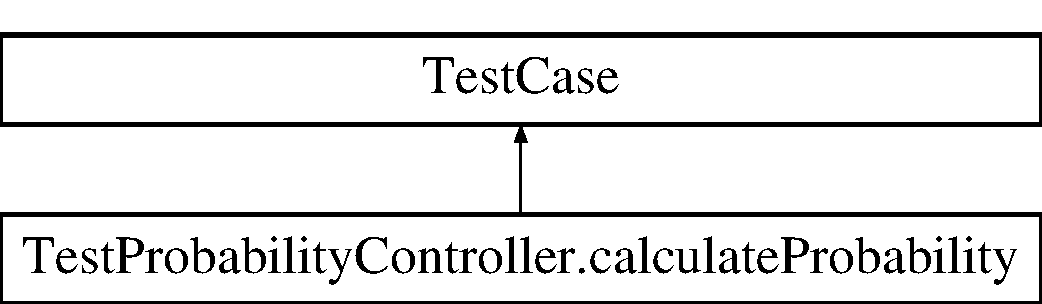
\includegraphics[height=2.000000cm]{class_test_probability_controller_1_1calculate_probability}
\end{center}
\end{figure}
\subsection*{Public Member Functions}
\begin{DoxyCompactItemize}
\item 
\mbox{\Hypertarget{class_test_probability_controller_1_1calculate_probability_a83dac9fb4705312b828a213df201de70}\label{class_test_probability_controller_1_1calculate_probability_a83dac9fb4705312b828a213df201de70}} 
def {\bfseries test\+\_\+\+Calculate\+Probability} (self)
\item 
\mbox{\Hypertarget{class_test_probability_controller_1_1calculate_probability_a8611411d74024a9f7dd981d5ddd5217b}\label{class_test_probability_controller_1_1calculate_probability_a8611411d74024a9f7dd981d5ddd5217b}} 
def {\bfseries test\+\_\+generate\+Probability} (self)
\end{DoxyCompactItemize}


The documentation for this class was generated from the following file\+:\begin{DoxyCompactItemize}
\item 
tests/unit\+Test/Test\+Probability\+Controller.\+py\end{DoxyCompactItemize}

\hypertarget{class_care_model_1_1_care_model}{}\section{Care\+Model.\+Care\+Model Class Reference}
\label{class_care_model_1_1_care_model}\index{Care\+Model.\+Care\+Model@{Care\+Model.\+Care\+Model}}
\subsection*{Public Member Functions}
\begin{DoxyCompactItemize}
\item 
def \mbox{\hyperlink{class_care_model_1_1_care_model_a89ed2bb8eb519313f953b5400fadf0e5}{\+\_\+\+\_\+init\+\_\+\+\_\+}} (self)
\end{DoxyCompactItemize}
\subsection*{Public Attributes}
\begin{DoxyCompactItemize}
\item 
\mbox{\Hypertarget{class_care_model_1_1_care_model_a1d587f35cbf47cd81d9a9cd5420e1590}\label{class_care_model_1_1_care_model_a1d587f35cbf47cd81d9a9cd5420e1590}} 
{\bfseries id\+Care}
\item 
\mbox{\Hypertarget{class_care_model_1_1_care_model_afbeacc40fa3fbedaebf724a0c269177f}\label{class_care_model_1_1_care_model_afbeacc40fa3fbedaebf724a0c269177f}} 
{\bfseries capacity}
\end{DoxyCompactItemize}


\subsection{Detailed Description}
\begin{DoxyVerb}Description: cette classe est modèle de centre d'accueil
Attributs:
    idCare: (int) l'identifiant de centre d'accueil
    capacity: (int) la capacité de centre d'accueil
\end{DoxyVerb}
 

\subsection{Constructor \& Destructor Documentation}
\mbox{\Hypertarget{class_care_model_1_1_care_model_a89ed2bb8eb519313f953b5400fadf0e5}\label{class_care_model_1_1_care_model_a89ed2bb8eb519313f953b5400fadf0e5}} 
\index{Care\+Model\+::\+Care\+Model@{Care\+Model\+::\+Care\+Model}!\+\_\+\+\_\+init\+\_\+\+\_\+@{\+\_\+\+\_\+init\+\_\+\+\_\+}}
\index{\+\_\+\+\_\+init\+\_\+\+\_\+@{\+\_\+\+\_\+init\+\_\+\+\_\+}!Care\+Model\+::\+Care\+Model@{Care\+Model\+::\+Care\+Model}}
\subsubsection{\texorpdfstring{\+\_\+\+\_\+init\+\_\+\+\_\+()}{\_\_init\_\_()}}
{\footnotesize\ttfamily def Care\+Model.\+Care\+Model.\+\_\+\+\_\+init\+\_\+\+\_\+ (\begin{DoxyParamCaption}\item[{}]{self }\end{DoxyParamCaption})}

\begin{DoxyVerb}Description: cette méthode est le constructeur de la classe CareModel
\end{DoxyVerb}
 

The documentation for this class was generated from the following file\+:\begin{DoxyCompactItemize}
\item 
models/data/Care\+Model.\+py\end{DoxyCompactItemize}

\hypertarget{class_file_controller_1_1_file_controller}{}\section{File\+Controller.\+File\+Controller Class Reference}
\label{class_file_controller_1_1_file_controller}\index{File\+Controller.\+File\+Controller@{File\+Controller.\+File\+Controller}}
\subsection*{Public Member Functions}
\begin{DoxyCompactItemize}
\item 
def \mbox{\hyperlink{class_file_controller_1_1_file_controller_a2302794d8bc553158b300c868dcc32c1}{read\+Building\+File}} (self, building\+Filename)
\item 
def \mbox{\hyperlink{class_file_controller_1_1_file_controller_a29b92a4d19263d13732a9edf7d218602}{read\+Care\+File}} (self, care\+Filename)
\item 
def \mbox{\hyperlink{class_file_controller_1_1_file_controller_a77fe65432e567dc86472b95759db1ee7}{read\+Distance\+File}} (self, distance\+Filename)
\item 
def \mbox{\hyperlink{class_file_controller_1_1_file_controller_a5d023bfee30423bd602d153f08f89910}{write\+Solution\+File}} (self, solution\+Filename, best\+Solution, instance)
\item 
def \mbox{\hyperlink{class_file_controller_1_1_file_controller_add13ed4f13f217efae17bd3f2e0f1563}{write\+Quality\+File}} (self, best\+Quality\+Of\+Each\+Iteration\+List, average\+Quality\+Of\+Each\+Iteration\+List)
\end{DoxyCompactItemize}


\subsection{Detailed Description}
\begin{DoxyVerb}Description: cette classe est le controleur de fichier, y compris la lecture et l'écriture
Attribut: rien
\end{DoxyVerb}
 

\subsection{Member Function Documentation}
\mbox{\Hypertarget{class_file_controller_1_1_file_controller_a2302794d8bc553158b300c868dcc32c1}\label{class_file_controller_1_1_file_controller_a2302794d8bc553158b300c868dcc32c1}} 
\index{File\+Controller\+::\+File\+Controller@{File\+Controller\+::\+File\+Controller}!read\+Building\+File@{read\+Building\+File}}
\index{read\+Building\+File@{read\+Building\+File}!File\+Controller\+::\+File\+Controller@{File\+Controller\+::\+File\+Controller}}
\subsubsection{\texorpdfstring{read\+Building\+File()}{readBuildingFile()}}
{\footnotesize\ttfamily def File\+Controller.\+File\+Controller.\+read\+Building\+File (\begin{DoxyParamCaption}\item[{}]{self,  }\item[{}]{building\+Filename }\end{DoxyParamCaption})}

\begin{DoxyVerb}Description: cette méthode est pour lire le fichier de bâtiment
:param buildingFilename: (String) le nom du fichier de bâtiment
:return: buildingContentList: (String[]) la liste de lignes du fichier de bâtiment
\end{DoxyVerb}
 \mbox{\Hypertarget{class_file_controller_1_1_file_controller_a29b92a4d19263d13732a9edf7d218602}\label{class_file_controller_1_1_file_controller_a29b92a4d19263d13732a9edf7d218602}} 
\index{File\+Controller\+::\+File\+Controller@{File\+Controller\+::\+File\+Controller}!read\+Care\+File@{read\+Care\+File}}
\index{read\+Care\+File@{read\+Care\+File}!File\+Controller\+::\+File\+Controller@{File\+Controller\+::\+File\+Controller}}
\subsubsection{\texorpdfstring{read\+Care\+File()}{readCareFile()}}
{\footnotesize\ttfamily def File\+Controller.\+File\+Controller.\+read\+Care\+File (\begin{DoxyParamCaption}\item[{}]{self,  }\item[{}]{care\+Filename }\end{DoxyParamCaption})}

\begin{DoxyVerb}Description: cette méthode est pour lire le fichier de centre d'accueil(care)
:param careFilename: (String) le nom du fichier care
:return: careContentList: (String[]) la liste de lignes du fichier de care
\end{DoxyVerb}
 \mbox{\Hypertarget{class_file_controller_1_1_file_controller_a77fe65432e567dc86472b95759db1ee7}\label{class_file_controller_1_1_file_controller_a77fe65432e567dc86472b95759db1ee7}} 
\index{File\+Controller\+::\+File\+Controller@{File\+Controller\+::\+File\+Controller}!read\+Distance\+File@{read\+Distance\+File}}
\index{read\+Distance\+File@{read\+Distance\+File}!File\+Controller\+::\+File\+Controller@{File\+Controller\+::\+File\+Controller}}
\subsubsection{\texorpdfstring{read\+Distance\+File()}{readDistanceFile()}}
{\footnotesize\ttfamily def File\+Controller.\+File\+Controller.\+read\+Distance\+File (\begin{DoxyParamCaption}\item[{}]{self,  }\item[{}]{distance\+Filename }\end{DoxyParamCaption})}

\begin{DoxyVerb}Description: cette méthode est pour lire le fichier de distance
:param distanceFilename: (String) le nom du fichier distance
:return: distanceContentList: (String[]) la liste de lignes du fichier de distance
\end{DoxyVerb}
 \mbox{\Hypertarget{class_file_controller_1_1_file_controller_add13ed4f13f217efae17bd3f2e0f1563}\label{class_file_controller_1_1_file_controller_add13ed4f13f217efae17bd3f2e0f1563}} 
\index{File\+Controller\+::\+File\+Controller@{File\+Controller\+::\+File\+Controller}!write\+Quality\+File@{write\+Quality\+File}}
\index{write\+Quality\+File@{write\+Quality\+File}!File\+Controller\+::\+File\+Controller@{File\+Controller\+::\+File\+Controller}}
\subsubsection{\texorpdfstring{write\+Quality\+File()}{writeQualityFile()}}
{\footnotesize\ttfamily def File\+Controller.\+File\+Controller.\+write\+Quality\+File (\begin{DoxyParamCaption}\item[{}]{self,  }\item[{}]{best\+Quality\+Of\+Each\+Iteration\+List,  }\item[{}]{average\+Quality\+Of\+Each\+Iteration\+List }\end{DoxyParamCaption})}

\begin{DoxyVerb}Description: cette méthode est pour écrire les qualités des meilleures solutions de chaque itération et
        les qualités moyennes des solutions de chaque itération dans le fichier de qualité
:param bestQualityOfEachIterationList: (float[]) la liste de qualités des meilleures solutions de chaque itération
:param averageQualityOfEachIterationList: (float[]) la liste de qualités moyennes de solutions de chaque itération
:return: rien
\end{DoxyVerb}
 \mbox{\Hypertarget{class_file_controller_1_1_file_controller_a5d023bfee30423bd602d153f08f89910}\label{class_file_controller_1_1_file_controller_a5d023bfee30423bd602d153f08f89910}} 
\index{File\+Controller\+::\+File\+Controller@{File\+Controller\+::\+File\+Controller}!write\+Solution\+File@{write\+Solution\+File}}
\index{write\+Solution\+File@{write\+Solution\+File}!File\+Controller\+::\+File\+Controller@{File\+Controller\+::\+File\+Controller}}
\subsubsection{\texorpdfstring{write\+Solution\+File()}{writeSolutionFile()}}
{\footnotesize\ttfamily def File\+Controller.\+File\+Controller.\+write\+Solution\+File (\begin{DoxyParamCaption}\item[{}]{self,  }\item[{}]{solution\+Filename,  }\item[{}]{best\+Solution,  }\item[{}]{instance }\end{DoxyParamCaption})}

\begin{DoxyVerb}Description: cette méthode est pour écrire la meilleure solutions dans le fichier de solution
:param solutionFilename: (String) le nom du fichier de solution
:param bestSolution: (l'object de la classe de SolutionModel) la meilleure solutions
:param instance: (l'objet de la classe de InstanceModel) l'instance pour ce projet
:return: rien
\end{DoxyVerb}
 

The documentation for this class was generated from the following file\+:\begin{DoxyCompactItemize}
\item 
controllers/File\+Controller.\+py\end{DoxyCompactItemize}

\hypertarget{class_instance_controller_1_1_instance_controller}{}\section{Instance\+Controller.\+Instance\+Controller Class Reference}
\label{class_instance_controller_1_1_instance_controller}\index{Instance\+Controller.\+Instance\+Controller@{Instance\+Controller.\+Instance\+Controller}}
\subsection*{Public Member Functions}
\begin{DoxyCompactItemize}
\item 
def \mbox{\hyperlink{class_instance_controller_1_1_instance_controller_a03bb3fbe1839d3b293f52105f8af0165}{\+\_\+\+\_\+init\+\_\+\+\_\+}} (self)
\item 
def \mbox{\hyperlink{class_instance_controller_1_1_instance_controller_aabe70fc23070b14aef590f99ac1c6296}{construct\+Instance}} (self, ant\+Quantity, building\+File\+Name, care\+File\+Name, distance\+File\+Name)
\item 
def \mbox{\hyperlink{class_instance_controller_1_1_instance_controller_a73f6a84881bc711978453e1af10fbb15}{solve\+Problem}} (self, iteration\+Times, care\+Effect\+Radius, solution\+File\+Name)
\end{DoxyCompactItemize}
\subsection*{Public Attributes}
\begin{DoxyCompactItemize}
\item 
\mbox{\Hypertarget{class_instance_controller_1_1_instance_controller_abaec6276d2033156730519a8a7f00aba}\label{class_instance_controller_1_1_instance_controller_abaec6276d2033156730519a8a7f00aba}} 
{\bfseries instance}
\end{DoxyCompactItemize}


\subsection{Detailed Description}
\begin{DoxyVerb}Description: cette classe est la controleur de instance de projet
Attribut:
    instance: (l'objet de la classe InstanceModel) l'instance pour ce projet
\end{DoxyVerb}
 

\subsection{Constructor \& Destructor Documentation}
\mbox{\Hypertarget{class_instance_controller_1_1_instance_controller_a03bb3fbe1839d3b293f52105f8af0165}\label{class_instance_controller_1_1_instance_controller_a03bb3fbe1839d3b293f52105f8af0165}} 
\index{Instance\+Controller\+::\+Instance\+Controller@{Instance\+Controller\+::\+Instance\+Controller}!\+\_\+\+\_\+init\+\_\+\+\_\+@{\+\_\+\+\_\+init\+\_\+\+\_\+}}
\index{\+\_\+\+\_\+init\+\_\+\+\_\+@{\+\_\+\+\_\+init\+\_\+\+\_\+}!Instance\+Controller\+::\+Instance\+Controller@{Instance\+Controller\+::\+Instance\+Controller}}
\subsubsection{\texorpdfstring{\+\_\+\+\_\+init\+\_\+\+\_\+()}{\_\_init\_\_()}}
{\footnotesize\ttfamily def Instance\+Controller.\+Instance\+Controller.\+\_\+\+\_\+init\+\_\+\+\_\+ (\begin{DoxyParamCaption}\item[{}]{self }\end{DoxyParamCaption})}

\begin{DoxyVerb}Description: cette méthode est le constructeur de la classe InstanceController
\end{DoxyVerb}
 

\subsection{Member Function Documentation}
\mbox{\Hypertarget{class_instance_controller_1_1_instance_controller_aabe70fc23070b14aef590f99ac1c6296}\label{class_instance_controller_1_1_instance_controller_aabe70fc23070b14aef590f99ac1c6296}} 
\index{Instance\+Controller\+::\+Instance\+Controller@{Instance\+Controller\+::\+Instance\+Controller}!construct\+Instance@{construct\+Instance}}
\index{construct\+Instance@{construct\+Instance}!Instance\+Controller\+::\+Instance\+Controller@{Instance\+Controller\+::\+Instance\+Controller}}
\subsubsection{\texorpdfstring{construct\+Instance()}{constructInstance()}}
{\footnotesize\ttfamily def Instance\+Controller.\+Instance\+Controller.\+construct\+Instance (\begin{DoxyParamCaption}\item[{}]{self,  }\item[{}]{ant\+Quantity,  }\item[{}]{building\+File\+Name,  }\item[{}]{care\+File\+Name,  }\item[{}]{distance\+File\+Name }\end{DoxyParamCaption})}

\begin{DoxyVerb}Description: cette classe est pour construire l'instance de projet
:param antQuantity: (int) le nombre de fourmis
:param buildingFileName: (String) le nom du fichier de bâtiment
:param careFileName: (String) le nom du fichier de care
:param distanceFileName: (String) le nom du fichier de distance
:return: rien
\end{DoxyVerb}
 \mbox{\Hypertarget{class_instance_controller_1_1_instance_controller_a73f6a84881bc711978453e1af10fbb15}\label{class_instance_controller_1_1_instance_controller_a73f6a84881bc711978453e1af10fbb15}} 
\index{Instance\+Controller\+::\+Instance\+Controller@{Instance\+Controller\+::\+Instance\+Controller}!solve\+Problem@{solve\+Problem}}
\index{solve\+Problem@{solve\+Problem}!Instance\+Controller\+::\+Instance\+Controller@{Instance\+Controller\+::\+Instance\+Controller}}
\subsubsection{\texorpdfstring{solve\+Problem()}{solveProblem()}}
{\footnotesize\ttfamily def Instance\+Controller.\+Instance\+Controller.\+solve\+Problem (\begin{DoxyParamCaption}\item[{}]{self,  }\item[{}]{iteration\+Times,  }\item[{}]{care\+Effect\+Radius,  }\item[{}]{solution\+File\+Name }\end{DoxyParamCaption})}

\begin{DoxyVerb}Description: cette méthode fournit la service de résoudre le problème
:param iterationTimes: (int) la fois d'itération
:param careEffectRadius: (int) le rayon d'attraction initial pour les cares
:param solutionFileName: le nom du fichier de solution qui enregistre la meilleure solution à la fin
:return: rien
\end{DoxyVerb}
 

The documentation for this class was generated from the following file\+:\begin{DoxyCompactItemize}
\item 
controllers/Instance\+Controller.\+py\end{DoxyCompactItemize}

\hypertarget{class_instance_model_1_1_instance_model}{}\section{Instance\+Model.\+Instance\+Model Class Reference}
\label{class_instance_model_1_1_instance_model}\index{Instance\+Model.\+Instance\+Model@{Instance\+Model.\+Instance\+Model}}
\subsection*{Public Member Functions}
\begin{DoxyCompactItemize}
\item 
def \mbox{\hyperlink{class_instance_model_1_1_instance_model_a1dc30e37013930d2e46caa7041298157}{\+\_\+\+\_\+init\+\_\+\+\_\+}} (self)
\end{DoxyCompactItemize}
\subsection*{Public Attributes}
\begin{DoxyCompactItemize}
\item 
\mbox{\Hypertarget{class_instance_model_1_1_instance_model_a5396b60a560d6fb125b7a884ac9e0dd5}\label{class_instance_model_1_1_instance_model_a5396b60a560d6fb125b7a884ac9e0dd5}} 
{\bfseries building\+List}
\item 
\mbox{\Hypertarget{class_instance_model_1_1_instance_model_a0ebf216fd055c6bf4aa3370a447f807b}\label{class_instance_model_1_1_instance_model_a0ebf216fd055c6bf4aa3370a447f807b}} 
{\bfseries care\+List}
\item 
\mbox{\Hypertarget{class_instance_model_1_1_instance_model_a5623321d9d653e37342c0bba9bde37d4}\label{class_instance_model_1_1_instance_model_a5623321d9d653e37342c0bba9bde37d4}} 
{\bfseries distance\+Matrix}
\item 
\mbox{\Hypertarget{class_instance_model_1_1_instance_model_a33c898c982f3a6a2ad1bcefb65768b8b}\label{class_instance_model_1_1_instance_model_a33c898c982f3a6a2ad1bcefb65768b8b}} 
{\bfseries pheromone\+Node\+List}
\item 
\mbox{\Hypertarget{class_instance_model_1_1_instance_model_a158d8dff7d7fdc3f99be3366a599389e}\label{class_instance_model_1_1_instance_model_a158d8dff7d7fdc3f99be3366a599389e}} 
{\bfseries pheromone\+Edge\+Matrix}
\item 
\mbox{\Hypertarget{class_instance_model_1_1_instance_model_abee0cc01b02603e5f42b60bafa6281f7}\label{class_instance_model_1_1_instance_model_abee0cc01b02603e5f42b60bafa6281f7}} 
{\bfseries ant\+List}
\end{DoxyCompactItemize}


\subsection{Detailed Description}
\begin{DoxyVerb}Description: cette class est le modèle d'instance pour ce projet
Attributs:
    buildingList: (BuildingModel[]) la liste de bâtiments
    careList: (CareList[]) la liste de cares
    distanceMatrix: (float[][]) la matrice de distances entre chaque bâtiment et chaque care
    pheromoneNodeList: (PheromoneNode[]) la liste de phéromones déposée sur le nœud de bâtiment
    pheromoneEdgeMatrix: (PheromoneEdge[][]) la  matrice de phéromones déposée sur l'arc entre le batiments et le case
    antList: (AntModel[]) la liste de fourmis
\end{DoxyVerb}
 

\subsection{Constructor \& Destructor Documentation}
\mbox{\Hypertarget{class_instance_model_1_1_instance_model_a1dc30e37013930d2e46caa7041298157}\label{class_instance_model_1_1_instance_model_a1dc30e37013930d2e46caa7041298157}} 
\index{Instance\+Model\+::\+Instance\+Model@{Instance\+Model\+::\+Instance\+Model}!\+\_\+\+\_\+init\+\_\+\+\_\+@{\+\_\+\+\_\+init\+\_\+\+\_\+}}
\index{\+\_\+\+\_\+init\+\_\+\+\_\+@{\+\_\+\+\_\+init\+\_\+\+\_\+}!Instance\+Model\+::\+Instance\+Model@{Instance\+Model\+::\+Instance\+Model}}
\subsubsection{\texorpdfstring{\+\_\+\+\_\+init\+\_\+\+\_\+()}{\_\_init\_\_()}}
{\footnotesize\ttfamily def Instance\+Model.\+Instance\+Model.\+\_\+\+\_\+init\+\_\+\+\_\+ (\begin{DoxyParamCaption}\item[{}]{self }\end{DoxyParamCaption})}

\begin{DoxyVerb}Desciption: cette méthode est le constructeur de la classe InstanceModel
\end{DoxyVerb}
 

The documentation for this class was generated from the following file\+:\begin{DoxyCompactItemize}
\item 
models/instance/Instance\+Model.\+py\end{DoxyCompactItemize}

\hypertarget{class_pheromone_edge_1_1_pheromone_edge}{}\section{Pheromone\+Edge.\+Pheromone\+Edge Class Reference}
\label{class_pheromone_edge_1_1_pheromone_edge}\index{Pheromone\+Edge.\+Pheromone\+Edge@{Pheromone\+Edge.\+Pheromone\+Edge}}
Inheritance diagram for Pheromone\+Edge.\+Pheromone\+Edge\+:\begin{figure}[H]
\begin{center}
\leavevmode
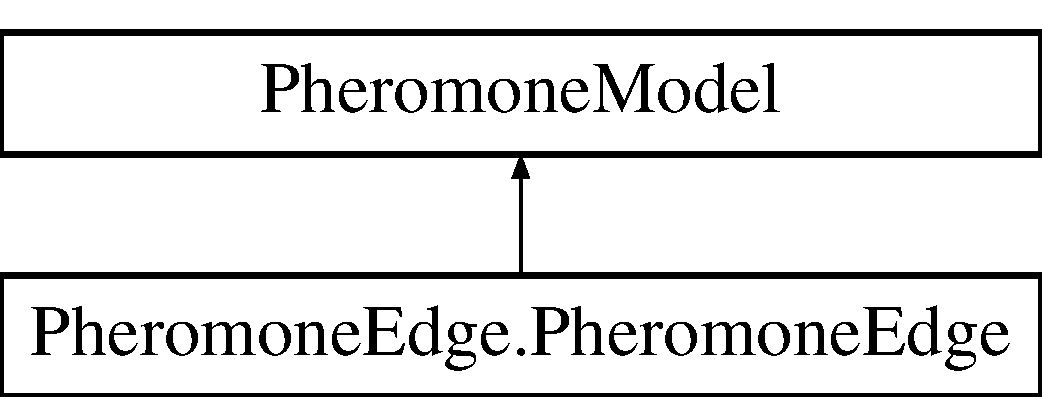
\includegraphics[height=2.000000cm]{class_pheromone_edge_1_1_pheromone_edge}
\end{center}
\end{figure}
\subsection*{Public Member Functions}
\begin{DoxyCompactItemize}
\item 
def \mbox{\hyperlink{class_pheromone_edge_1_1_pheromone_edge_add7daf216e9ce9c5ac6b5991036fe615}{\+\_\+\+\_\+init\+\_\+\+\_\+}} (self)
\end{DoxyCompactItemize}


\subsection{Detailed Description}
\begin{DoxyVerb}Description: cette classe est le modèle de phéromone qui est déposée sur les arcs entre le bâtiment et le care
Classe parent: PeromoneModel (cette classe hérite de la classe PeromoneModel)
Attributs:
    Tous les attributs de classe parent
\end{DoxyVerb}
 

\subsection{Constructor \& Destructor Documentation}
\mbox{\Hypertarget{class_pheromone_edge_1_1_pheromone_edge_add7daf216e9ce9c5ac6b5991036fe615}\label{class_pheromone_edge_1_1_pheromone_edge_add7daf216e9ce9c5ac6b5991036fe615}} 
\index{Pheromone\+Edge\+::\+Pheromone\+Edge@{Pheromone\+Edge\+::\+Pheromone\+Edge}!\+\_\+\+\_\+init\+\_\+\+\_\+@{\+\_\+\+\_\+init\+\_\+\+\_\+}}
\index{\+\_\+\+\_\+init\+\_\+\+\_\+@{\+\_\+\+\_\+init\+\_\+\+\_\+}!Pheromone\+Edge\+::\+Pheromone\+Edge@{Pheromone\+Edge\+::\+Pheromone\+Edge}}
\subsubsection{\texorpdfstring{\+\_\+\+\_\+init\+\_\+\+\_\+()}{\_\_init\_\_()}}
{\footnotesize\ttfamily def Pheromone\+Edge.\+Pheromone\+Edge.\+\_\+\+\_\+init\+\_\+\+\_\+ (\begin{DoxyParamCaption}\item[{}]{self }\end{DoxyParamCaption})}

\begin{DoxyVerb}Desciption: cette méthode est le constructeur de la classe PheromoneEdge
\end{DoxyVerb}
 

The documentation for this class was generated from the following file\+:\begin{DoxyCompactItemize}
\item 
models/pheromone/Pheromone\+Edge.\+py\end{DoxyCompactItemize}

\hypertarget{class_pheromone_model_1_1_pheromone_model}{}\section{Pheromone\+Model.\+Pheromone\+Model Class Reference}
\label{class_pheromone_model_1_1_pheromone_model}\index{Pheromone\+Model.\+Pheromone\+Model@{Pheromone\+Model.\+Pheromone\+Model}}
\subsection*{Public Member Functions}
\begin{DoxyCompactItemize}
\item 
def \mbox{\hyperlink{class_pheromone_model_1_1_pheromone_model_a7d692c818254359644c81f058dc89ba0}{\+\_\+\+\_\+init\+\_\+\+\_\+}} (self)
\end{DoxyCompactItemize}
\subsection*{Public Attributes}
\begin{DoxyCompactItemize}
\item 
\mbox{\Hypertarget{class_pheromone_model_1_1_pheromone_model_ad9abf0a724e3e5dfd06abb3c74cf15d5}\label{class_pheromone_model_1_1_pheromone_model_ad9abf0a724e3e5dfd06abb3c74cf15d5}} 
{\bfseries eta}
\item 
\mbox{\Hypertarget{class_pheromone_model_1_1_pheromone_model_a2d2e77f8db0cb747d32f2889eac15fef}\label{class_pheromone_model_1_1_pheromone_model_a2d2e77f8db0cb747d32f2889eac15fef}} 
{\bfseries tau}
\item 
\mbox{\Hypertarget{class_pheromone_model_1_1_pheromone_model_ac660c2c6a81ad79fbb577de1f8ae6563}\label{class_pheromone_model_1_1_pheromone_model_ac660c2c6a81ad79fbb577de1f8ae6563}} 
{\bfseries delta\+Tau}
\item 
\mbox{\Hypertarget{class_pheromone_model_1_1_pheromone_model_acd496c31c606a05fafdcaa16267fa3d5}\label{class_pheromone_model_1_1_pheromone_model_acd496c31c606a05fafdcaa16267fa3d5}} 
{\bfseries rho}
\end{DoxyCompactItemize}


\subsection{Detailed Description}
\begin{DoxyVerb}Description: cette classe est le modèle de phéromone
Attributs:
    eta: (float) la désirabilité de mouvement
    tau: (float) la quantité de phéromones existant
    deltaTau: (float) la quantité de phéromones déposés lors que la fourmi prend un nœud ou un arc
    rho: (float) le taux d'évaporation de phéromones
\end{DoxyVerb}
 

\subsection{Constructor \& Destructor Documentation}
\mbox{\Hypertarget{class_pheromone_model_1_1_pheromone_model_a7d692c818254359644c81f058dc89ba0}\label{class_pheromone_model_1_1_pheromone_model_a7d692c818254359644c81f058dc89ba0}} 
\index{Pheromone\+Model\+::\+Pheromone\+Model@{Pheromone\+Model\+::\+Pheromone\+Model}!\+\_\+\+\_\+init\+\_\+\+\_\+@{\+\_\+\+\_\+init\+\_\+\+\_\+}}
\index{\+\_\+\+\_\+init\+\_\+\+\_\+@{\+\_\+\+\_\+init\+\_\+\+\_\+}!Pheromone\+Model\+::\+Pheromone\+Model@{Pheromone\+Model\+::\+Pheromone\+Model}}
\subsubsection{\texorpdfstring{\+\_\+\+\_\+init\+\_\+\+\_\+()}{\_\_init\_\_()}}
{\footnotesize\ttfamily def Pheromone\+Model.\+Pheromone\+Model.\+\_\+\+\_\+init\+\_\+\+\_\+ (\begin{DoxyParamCaption}\item[{}]{self }\end{DoxyParamCaption})}

\begin{DoxyVerb}Desciption: cette méthode est le constructeur de la classe PheromoneModel
\end{DoxyVerb}
 

The documentation for this class was generated from the following file\+:\begin{DoxyCompactItemize}
\item 
models/pheromone/Pheromone\+Model.\+py\end{DoxyCompactItemize}

\hypertarget{class_pheromone_node_1_1_pheromone_node}{}\section{Pheromone\+Node.\+Pheromone\+Node Class Reference}
\label{class_pheromone_node_1_1_pheromone_node}\index{Pheromone\+Node.\+Pheromone\+Node@{Pheromone\+Node.\+Pheromone\+Node}}
Inheritance diagram for Pheromone\+Node.\+Pheromone\+Node\+:\begin{figure}[H]
\begin{center}
\leavevmode
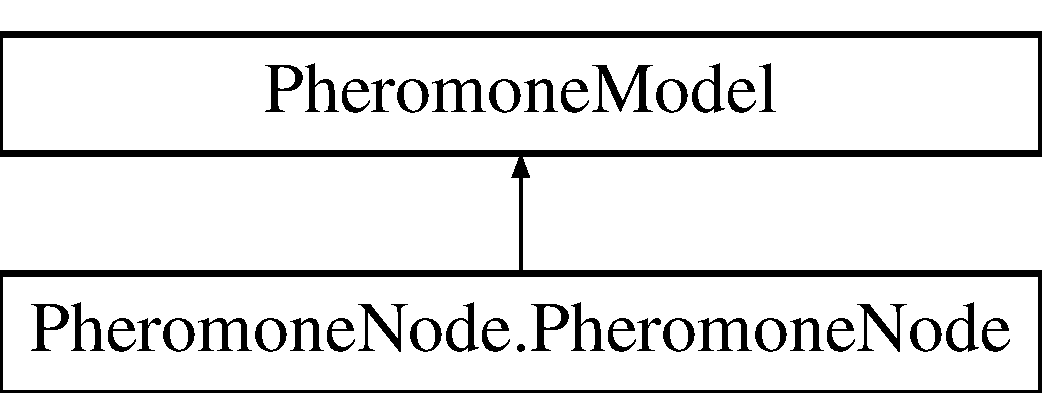
\includegraphics[height=2.000000cm]{class_pheromone_node_1_1_pheromone_node}
\end{center}
\end{figure}
\subsection*{Public Member Functions}
\begin{DoxyCompactItemize}
\item 
def \mbox{\hyperlink{class_pheromone_node_1_1_pheromone_node_a7a55026a7737706b59449032e96fe695}{\+\_\+\+\_\+init\+\_\+\+\_\+}} (self)
\end{DoxyCompactItemize}


\subsection{Detailed Description}
\begin{DoxyVerb}Description: cette classe est le modèle de phéromone qui est déposée sur les nœuds de bâtiment
Classe parent: PeromoneModel (cette classe hérite de la classe PeromoneModel)
Attributs:
    Tous les attributs de classe parent
\end{DoxyVerb}
 

\subsection{Constructor \& Destructor Documentation}
\mbox{\Hypertarget{class_pheromone_node_1_1_pheromone_node_a7a55026a7737706b59449032e96fe695}\label{class_pheromone_node_1_1_pheromone_node_a7a55026a7737706b59449032e96fe695}} 
\index{Pheromone\+Node\+::\+Pheromone\+Node@{Pheromone\+Node\+::\+Pheromone\+Node}!\+\_\+\+\_\+init\+\_\+\+\_\+@{\+\_\+\+\_\+init\+\_\+\+\_\+}}
\index{\+\_\+\+\_\+init\+\_\+\+\_\+@{\+\_\+\+\_\+init\+\_\+\+\_\+}!Pheromone\+Node\+::\+Pheromone\+Node@{Pheromone\+Node\+::\+Pheromone\+Node}}
\subsubsection{\texorpdfstring{\+\_\+\+\_\+init\+\_\+\+\_\+()}{\_\_init\_\_()}}
{\footnotesize\ttfamily def Pheromone\+Node.\+Pheromone\+Node.\+\_\+\+\_\+init\+\_\+\+\_\+ (\begin{DoxyParamCaption}\item[{}]{self }\end{DoxyParamCaption})}

\begin{DoxyVerb}Desciption: cette méthode est le constructeur de la classe PheromoneNode
\end{DoxyVerb}
 

The documentation for this class was generated from the following file\+:\begin{DoxyCompactItemize}
\item 
models/pheromone/Pheromone\+Node.\+py\end{DoxyCompactItemize}

\hypertarget{class_probability_controller_1_1_probability_controller}{}\section{Probability\+Controller.\+Probability\+Controller Class Reference}
\label{class_probability_controller_1_1_probability_controller}\index{Probability\+Controller.\+Probability\+Controller@{Probability\+Controller.\+Probability\+Controller}}
\subsection*{Public Member Functions}
\begin{DoxyCompactItemize}
\item 
def \mbox{\hyperlink{class_probability_controller_1_1_probability_controller_a842dac0f2f434e2ddab5d108c70e13fb}{calculate\+Probability}} (self, eta, tau, boolean\+List)
\item 
def \mbox{\hyperlink{class_probability_controller_1_1_probability_controller_a0cb0e1ffa81219cf1493859c897edb01}{generate\+Probability}} (self, id\+Probability\+List, probability\+List)
\end{DoxyCompactItemize}


\subsection{Detailed Description}
\begin{DoxyVerb}Description: cette classe est pour contrôler la probabilité lorsque les fourmis déplacent
Attributs: rien
\end{DoxyVerb}
 

\subsection{Member Function Documentation}
\mbox{\Hypertarget{class_probability_controller_1_1_probability_controller_a842dac0f2f434e2ddab5d108c70e13fb}\label{class_probability_controller_1_1_probability_controller_a842dac0f2f434e2ddab5d108c70e13fb}} 
\index{Probability\+Controller\+::\+Probability\+Controller@{Probability\+Controller\+::\+Probability\+Controller}!calculate\+Probability@{calculate\+Probability}}
\index{calculate\+Probability@{calculate\+Probability}!Probability\+Controller\+::\+Probability\+Controller@{Probability\+Controller\+::\+Probability\+Controller}}
\subsubsection{\texorpdfstring{calculate\+Probability()}{calculateProbability()}}
{\footnotesize\ttfamily def Probability\+Controller.\+Probability\+Controller.\+calculate\+Probability (\begin{DoxyParamCaption}\item[{}]{self,  }\item[{}]{eta,  }\item[{}]{tau,  }\item[{}]{boolean\+List }\end{DoxyParamCaption})}

\begin{DoxyVerb}Description: cette méthode est pour calculer la probabilité de déplacement
:param eta: (float) la désirabilité de déplacement
:param tau: (float) la quantité de phéromones existant sur un nœud de bâtiment ou un arc entre un bâtiment et un care
:param booleanList: (boolean[]) soit la liste qui marque si le bâtiment est déjà affecté, soit la liste qui marque si le care est plein
:return: probability: (float) la probabilité de déplacement calculée
\end{DoxyVerb}
 \mbox{\Hypertarget{class_probability_controller_1_1_probability_controller_a0cb0e1ffa81219cf1493859c897edb01}\label{class_probability_controller_1_1_probability_controller_a0cb0e1ffa81219cf1493859c897edb01}} 
\index{Probability\+Controller\+::\+Probability\+Controller@{Probability\+Controller\+::\+Probability\+Controller}!generate\+Probability@{generate\+Probability}}
\index{generate\+Probability@{generate\+Probability}!Probability\+Controller\+::\+Probability\+Controller@{Probability\+Controller\+::\+Probability\+Controller}}
\subsubsection{\texorpdfstring{generate\+Probability()}{generateProbability()}}
{\footnotesize\ttfamily def Probability\+Controller.\+Probability\+Controller.\+generate\+Probability (\begin{DoxyParamCaption}\item[{}]{self,  }\item[{}]{id\+Probability\+List,  }\item[{}]{probability\+List }\end{DoxyParamCaption})}

\begin{DoxyVerb}Description: cette méthode est pour sélectionner un événement qui correspond à une probabilité au hasard
:param idProbabilityList: (int[]) la séquence qui contient les identifiants de bâtiment ou de care
:param probabilityList: (float[]) la liste de probabilité de déplacement
:return: item: (int) l'identifiant de l'arcticle(bâtiment ou care) sélectionné au hasard selon les probabilités
\end{DoxyVerb}
 

The documentation for this class was generated from the following file\+:\begin{DoxyCompactItemize}
\item 
controllers/Probability\+Controller.\+py\end{DoxyCompactItemize}

\hypertarget{class_solution_model_1_1_solution_model}{}\section{Solution\+Model.\+Solution\+Model Class Reference}
\label{class_solution_model_1_1_solution_model}\index{Solution\+Model.\+Solution\+Model@{Solution\+Model.\+Solution\+Model}}
\subsection*{Public Member Functions}
\begin{DoxyCompactItemize}
\item 
def \mbox{\hyperlink{class_solution_model_1_1_solution_model_af442c5ef771172d03dec082d5de64a20}{\+\_\+\+\_\+init\+\_\+\+\_\+}} (self)
\end{DoxyCompactItemize}
\subsection*{Public Attributes}
\begin{DoxyCompactItemize}
\item 
\mbox{\Hypertarget{class_solution_model_1_1_solution_model_afed9b63c4bc32f081bd40040161036ac}\label{class_solution_model_1_1_solution_model_afed9b63c4bc32f081bd40040161036ac}} 
{\bfseries solution\+Array}
\item 
\mbox{\Hypertarget{class_solution_model_1_1_solution_model_aff0c87fed25d6998522a8ad3dacb1ce6}\label{class_solution_model_1_1_solution_model_aff0c87fed25d6998522a8ad3dacb1ce6}} 
{\bfseries quality}
\end{DoxyCompactItemize}


\subsection{Detailed Description}
\begin{DoxyVerb}Description: cette classe est le modèle de solution construite par chaque fourmi
Attributs:
    solutionArray: (int[]) le tableau d'une solution
    quality: (float) la qualité de solution
\end{DoxyVerb}
 

\subsection{Constructor \& Destructor Documentation}
\mbox{\Hypertarget{class_solution_model_1_1_solution_model_af442c5ef771172d03dec082d5de64a20}\label{class_solution_model_1_1_solution_model_af442c5ef771172d03dec082d5de64a20}} 
\index{Solution\+Model\+::\+Solution\+Model@{Solution\+Model\+::\+Solution\+Model}!\+\_\+\+\_\+init\+\_\+\+\_\+@{\+\_\+\+\_\+init\+\_\+\+\_\+}}
\index{\+\_\+\+\_\+init\+\_\+\+\_\+@{\+\_\+\+\_\+init\+\_\+\+\_\+}!Solution\+Model\+::\+Solution\+Model@{Solution\+Model\+::\+Solution\+Model}}
\subsubsection{\texorpdfstring{\+\_\+\+\_\+init\+\_\+\+\_\+()}{\_\_init\_\_()}}
{\footnotesize\ttfamily def Solution\+Model.\+Solution\+Model.\+\_\+\+\_\+init\+\_\+\+\_\+ (\begin{DoxyParamCaption}\item[{}]{self }\end{DoxyParamCaption})}

\begin{DoxyVerb}Description: cette méthode est le constructeur de la classe SolutionModel
\end{DoxyVerb}
 

The documentation for this class was generated from the following file\+:\begin{DoxyCompactItemize}
\item 
models/ant/Solution\+Model.\+py\end{DoxyCompactItemize}

\hypertarget{class_test_algorithm_controller_1_1_test_algorithm_controller}{}\section{Test\+Algorithm\+Controller.\+Test\+Algorithm\+Controller Class Reference}
\label{class_test_algorithm_controller_1_1_test_algorithm_controller}\index{Test\+Algorithm\+Controller.\+Test\+Algorithm\+Controller@{Test\+Algorithm\+Controller.\+Test\+Algorithm\+Controller}}
Inheritance diagram for Test\+Algorithm\+Controller.\+Test\+Algorithm\+Controller\+:\begin{figure}[H]
\begin{center}
\leavevmode
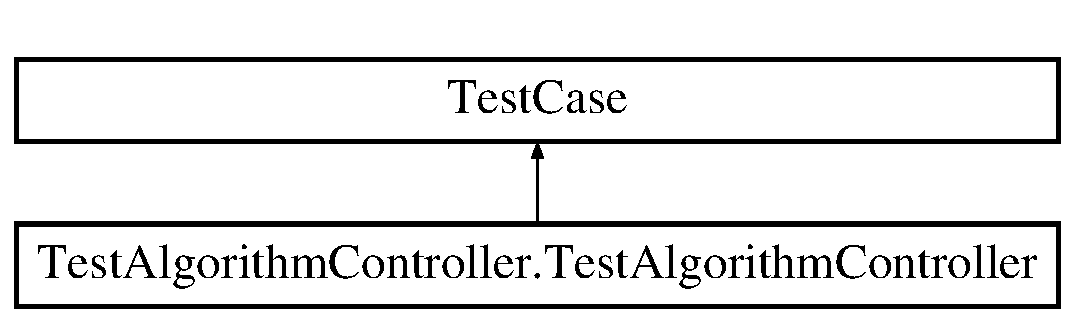
\includegraphics[height=2.000000cm]{class_test_algorithm_controller_1_1_test_algorithm_controller}
\end{center}
\end{figure}
\subsection*{Public Member Functions}
\begin{DoxyCompactItemize}
\item 
\mbox{\Hypertarget{class_test_algorithm_controller_1_1_test_algorithm_controller_a80501ce09022359dc79254b6439a468b}\label{class_test_algorithm_controller_1_1_test_algorithm_controller_a80501ce09022359dc79254b6439a468b}} 
def {\bfseries test\+\_\+merge\+\_\+sort} (self)
\item 
\mbox{\Hypertarget{class_test_algorithm_controller_1_1_test_algorithm_controller_a637e7050ee760c6fd7d6b6a8b0a3a034}\label{class_test_algorithm_controller_1_1_test_algorithm_controller_a637e7050ee760c6fd7d6b6a8b0a3a034}} 
def {\bfseries test\+\_\+sort\+Building\+Index\+For\+Each\+Care\+In\+Distance\+Matrix} (self)
\end{DoxyCompactItemize}


The documentation for this class was generated from the following file\+:\begin{DoxyCompactItemize}
\item 
tests/unit\+Test/Test\+Algorithm\+Controller.\+py\end{DoxyCompactItemize}

\hypertarget{class_test_file_controller_1_1_test_file_controller}{}\section{Test\+File\+Controller.\+Test\+File\+Controller Class Reference}
\label{class_test_file_controller_1_1_test_file_controller}\index{Test\+File\+Controller.\+Test\+File\+Controller@{Test\+File\+Controller.\+Test\+File\+Controller}}
Inheritance diagram for Test\+File\+Controller.\+Test\+File\+Controller\+:\begin{figure}[H]
\begin{center}
\leavevmode
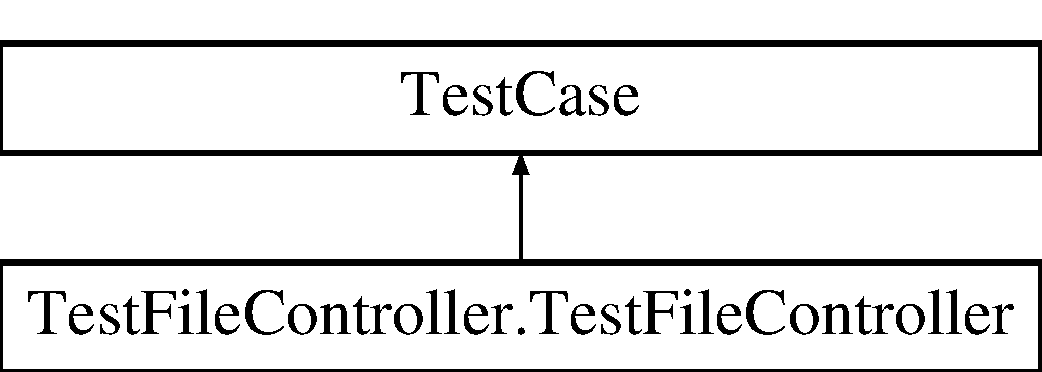
\includegraphics[height=2.000000cm]{class_test_file_controller_1_1_test_file_controller}
\end{center}
\end{figure}
\subsection*{Public Member Functions}
\begin{DoxyCompactItemize}
\item 
\mbox{\Hypertarget{class_test_file_controller_1_1_test_file_controller_a4459fe53869c56c33541fbfc63b340c6}\label{class_test_file_controller_1_1_test_file_controller_a4459fe53869c56c33541fbfc63b340c6}} 
def {\bfseries test\+\_\+\+Read\+Building\+File} (self)
\item 
\mbox{\Hypertarget{class_test_file_controller_1_1_test_file_controller_aee7a4d0bdc025d2963d9238b0036b999}\label{class_test_file_controller_1_1_test_file_controller_aee7a4d0bdc025d2963d9238b0036b999}} 
def {\bfseries test\+\_\+\+Read\+Care\+File} (self)
\item 
\mbox{\Hypertarget{class_test_file_controller_1_1_test_file_controller_a7e98fe3da36c09e0f9681761d6a42871}\label{class_test_file_controller_1_1_test_file_controller_a7e98fe3da36c09e0f9681761d6a42871}} 
def {\bfseries test\+\_\+\+Read\+Distance\+File} (self)
\end{DoxyCompactItemize}


The documentation for this class was generated from the following file\+:\begin{DoxyCompactItemize}
\item 
tests/unit\+Test/Test\+File\+Controller.\+py\end{DoxyCompactItemize}

\hypertarget{class_test_instance_controller_1_1_test_instance_controller}{}\section{Test\+Instance\+Controller.\+Test\+Instance\+Controller Class Reference}
\label{class_test_instance_controller_1_1_test_instance_controller}\index{Test\+Instance\+Controller.\+Test\+Instance\+Controller@{Test\+Instance\+Controller.\+Test\+Instance\+Controller}}
Inheritance diagram for Test\+Instance\+Controller.\+Test\+Instance\+Controller\+:\begin{figure}[H]
\begin{center}
\leavevmode
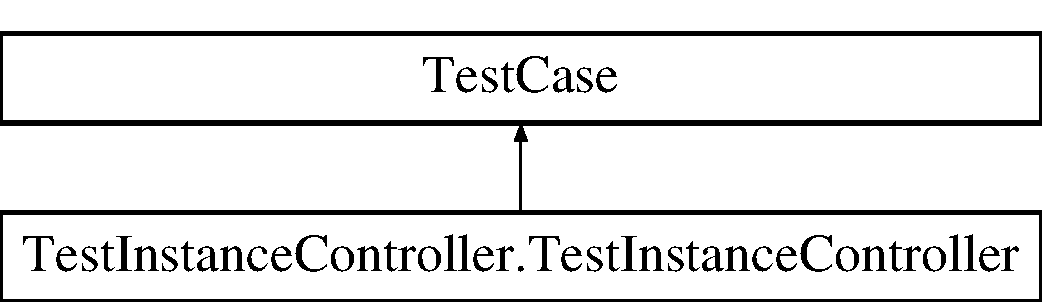
\includegraphics[height=2.000000cm]{class_test_instance_controller_1_1_test_instance_controller}
\end{center}
\end{figure}
\subsection*{Public Member Functions}
\begin{DoxyCompactItemize}
\item 
\mbox{\Hypertarget{class_test_instance_controller_1_1_test_instance_controller_a22d0c6acd66dcff8579c0eba5e863ee1}\label{class_test_instance_controller_1_1_test_instance_controller_a22d0c6acd66dcff8579c0eba5e863ee1}} 
def {\bfseries test\+\_\+construct\+Instance} (self)
\end{DoxyCompactItemize}


The documentation for this class was generated from the following file\+:\begin{DoxyCompactItemize}
\item 
tests/unit\+Test/Test\+Instance\+Controller.\+py\end{DoxyCompactItemize}

\hypertarget{class_test_parameters_1_1_test_parameters}{}\section{Test\+Parameters.\+Test\+Parameters Class Reference}
\label{class_test_parameters_1_1_test_parameters}\index{Test\+Parameters.\+Test\+Parameters@{Test\+Parameters.\+Test\+Parameters}}
\subsection*{Public Member Functions}
\begin{DoxyCompactItemize}
\item 
\mbox{\Hypertarget{class_test_parameters_1_1_test_parameters_a390dd3de3015f5d9b125ea92bd726d2a}\label{class_test_parameters_1_1_test_parameters_a390dd3de3015f5d9b125ea92bd726d2a}} 
def {\bfseries draw\+Figure} (self)
\end{DoxyCompactItemize}


The documentation for this class was generated from the following file\+:\begin{DoxyCompactItemize}
\item 
tests/functional\+Test/Test\+Parameters.\+py\end{DoxyCompactItemize}

\hypertarget{class_test_solution_1_1_test_solution}{}\section{Test\+Solution.\+Test\+Solution Class Reference}
\label{class_test_solution_1_1_test_solution}\index{Test\+Solution.\+Test\+Solution@{Test\+Solution.\+Test\+Solution}}
\subsection*{Public Member Functions}
\begin{DoxyCompactItemize}
\item 
\mbox{\Hypertarget{class_test_solution_1_1_test_solution_a6d1b573caf6cf311edc262c7bb4a1577}\label{class_test_solution_1_1_test_solution_a6d1b573caf6cf311edc262c7bb4a1577}} 
def {\bfseries draw\+Map} (self)
\end{DoxyCompactItemize}


The documentation for this class was generated from the following file\+:\begin{DoxyCompactItemize}
\item 
tests/functional\+Test/Test\+Solution.\+py\end{DoxyCompactItemize}

%--- End generated contents ---

% Index
\backmatter
\newpage
\phantomsection
\clearemptydoublepage
\addcontentsline{toc}{chapter}{Index}
\printindex

\end{document}
